%(BEGIN_QUESTION)
% Copyright 2008, Tony R. Kuphaldt, released under the Creative Commons Attribution License (v 1.0)
% This means you may do almost anything with this work of mine, so long as you give me proper credit

Beskriv hva utgangsspenningen i denne operasjonsforsterkerkretsen vil gjøre ved en konstant inngangsspenning på +2 volt:

$$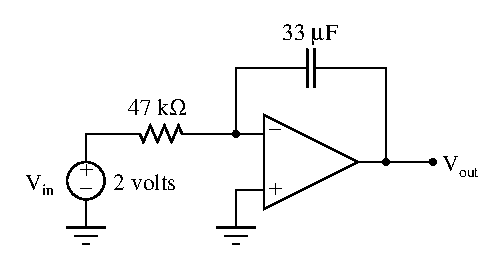
\includegraphics[width=15.5cm]{i01576x01.eps}$$

Vær så spesifikk som mulig i svaret ditt!

\underbar{file i01576}
%(END_QUESTION)





%(BEGIN_ANSWER)

Utgangsspenningen blir stadig mer negativ med en hastighet på -1.289 volt per sekund.

\vskip 10pt

Hint: husk ``Ohms lov'' for en kondensator, som knytter strøm til spenningsendring over tid,

$$i = C {du \over dt}$$

%(END_ANSWER)





%(BEGIN_NOTES)


\filbreak \vskip 20pt \vbox{\hrule \hbox{\strut \vrule{} {\bf Virtuell feilsøking} \vrule} \hrule}

\noindent
{\bf Forutsi virkningen av en gitt feil:} presenter hver av følgende feil for studentene, én om gangen, og la dem kommentere alle virkningene hver feil vil gi.

\begin{itemize}
\item{} Motstand har feilet åpen
\item{} Kondensator har feilet åpen
\item{} Motstand har feilet kortsluttet
\item{} Kondensator har feilet kortsluttet
\item{} Forbindelsen fra (+)-inngangen til jord har feilet åpen
\item{} Polariteten på $U_{in}$ er ved en feil snudd
\end{itemize}


\vskip 10pt


\noindent
{\bf Identifiser mulige/umulige feil:} presenter symptomer for studentene, og la dem deretter avgjøre om en rekke foreslåtte feil kan forklare alle symptomene. De skal forklare {\it hvorfor} eller {\it hvorfor ikke} for hver foreslåtte feil:

\begin{itemize}
\item{} Symptom: {\it }
\item{} 
\item{} 
\item{} 
\end{itemize}


\vskip 10pt


\noindent
{\bf Vurder nytten av gitte diagnostiske tester:} presenter symptomer for studentene, og foreslå deretter følgende diagnostiske tester én etter én. Studentene vurderer verdien av hver test og avgjør om den vil gi nyttig informasjon (dvs. fortelle oss noe vi ikke allerede vet). Studentene avgjør også hva ulike testresultater vil indikere om feilen, hvis noe:

\begin{itemize}
\item{} Symptom: {\it }
\item{}  -- {\bf Ja/Nei}
\item{}  -- {\bf Ja/Nei}
\end{itemize}


\vskip 10pt


\noindent
{\bf Diagnostiser en feil basert på gitte symptomer:} tenk deg at ??? feiler ??? i dette systemet (ikke avslør feilen for studentene!). Presenter operatørens observasjon(er), la studentene vurdere mulige feil og teststrategier, og gi dem deretter resultatene av testene de foreslår basert på følgende symptomer, helt til de har identifisert feilens natur og plassering korrekt:

\begin{itemize}
\item{} {\it }
\item{} 
\item{} 
\end{itemize}
%INDEX% Electronics review: integrator circuit

%(END_NOTES)
